\documentclass[10.5pt,a4paper]{article}
\usepackage[utf8]{inputenc}
\usepackage[T1]{fontenc}
\renewcommand{\contentsname}{Table des matières}
\usepackage{amsmath,amssymb}
\usepackage{geometry}
\geometry{margin=2cm}
\usepackage{tikz}
\usetikzlibrary{arrows.meta}
\usepackage{xcolor}
\usepackage{enumitem}
\usepackage{booktabs}
\usepackage{tabularx}
\usepackage{array}
\usepackage{mdframed}
\usepackage{hyperref}
\hypersetup{colorlinks=true,linkcolor=blue!50!black}

\definecolor{cbleu}{RGB}{25,80,180}
\definecolor{cvert}{RGB}{20,120,55}
\definecolor{crouge}{RGB}{190,30,30}
\definecolor{cgris}{RGB}{95,95,95}

\newmdenv[
  linecolor=cgris!60, backgroundcolor=cgris!6,
  linewidth=0.8pt, roundcorner=3pt, innermargin=8pt, innertopmargin=6pt, innerbottommargin=6pt,
  skipabove=8pt, skipbelow=8pt
]{enonce}

\newmdenv[
  linecolor=cvert, backgroundcolor=cvert!5,
  linewidth=1pt, roundcorner=4pt, innermargin=8pt, innertopmargin=6pt, innerbottommargin=6pt,
  skipabove=8pt, skipbelow=8pt
]{verif}

\newmdenv[
  linecolor=orange!70!black, backgroundcolor=orange!6,
  linewidth=1pt, roundcorner=4pt, innermargin=8pt, innertopmargin=6pt, innerbottommargin=6pt,
  skipabove=8pt, skipbelow=8pt
]{piege}

\newmdenv[
  linecolor=cbleu, backgroundcolor=cbleu!5,
  linewidth=1pt, roundcorner=4pt, innermargin=8pt, innertopmargin=6pt, innerbottommargin=6pt,
  skipabove=8pt, skipbelow=8pt
]{reflexe}

% --- environnement etape ---
\newcounter{et}[section]
\newcommand{\etape}[1]{%
  \refstepcounter{et}%
  \medskip\par\noindent
  {\color{cbleu}\bfseries Étape \theet\ --- #1}\par\nobreak\smallskip}
\newcommand{\pq}[1]{{\color{cgris}\itshape\small Pourquoi : #1\par}\smallskip}

\title{\textbf{Résoudre les exercices à la main}\\[3pt]
\large Marche à suivre détaillée, étape par étape}
\author{}
\date{}

\begin{document}
\maketitle
\vspace{-0.9cm}
\begin{center}
\small\itshape Chaque exercice type est refait entièrement à la main : l'ordre des étapes, la formule
utilisée, l'application numérique complète, et la raison de chaque geste.
\end{center}
\vspace{0.2cm}
\tableofcontents
\newpage

%=====================================================
\section{Avant de commencer : organiser sa feuille}

\begin{reflexe}
\textbf{Le réflexe, quel que soit l'exercice :} ne jamais se lancer dans un calcul avant d'avoir
\textbf{dessiné le cycle} et \textbf{tracé le tableau d'état}. 90 \% des erreurs viennent d'une
transformation mal identifiée, pas d'une erreur de calcul.
\end{reflexe}

\textbf{En haut de la feuille}, recopiez les données et convertissez tout de suite :
\begin{itemize}[leftmargin=1.4em,nosep]
\item toutes les \textbf{températures en K} ($T[\text{K}]=T[^\circ\text{C}]+273{,}15$) ;
\item les \textbf{pressions en Pa} ($1$ bar $=10^5$ Pa) ;
\item les \textbf{volumes en m}$^3$ ($1$ L $=10^{-3}$ m$^3$, $1$ cm$^3=10^{-6}$ m$^3$).
\end{itemize}

\textbf{Puis tracez ce tableau} (autant de colonnes que de points du cycle) :

\begin{center}
\renewcommand{\arraystretch}{1.5}
\begin{tabular}{@{}l|c|c|c|c|c@{}}
\toprule
& \textbf{A} & \textbf{B} & \textbf{C} & \textbf{D} & \textbf{E} \\
\midrule
$p$ [Pa] & & & & & \\
$V$ [m$^3$] & & & & & \\
$T$ [K] & & & & & \\
\bottomrule
\end{tabular}
\end{center}

\textbf{Et en dessous}, un second tableau pour les énergies :

\begin{center}
\renewcommand{\arraystretch}{1.5}
\begin{tabular}{@{}l|c|c|c|c@{}}
\toprule
& \textbf{A$\to$B} & \textbf{B$\to$C} & \textbf{C$\to$D} & \textbf{...} \\
\midrule
type de transfo & & & & \\
$W$ [J] & & & & \\
$Q$ [J] & & & & \\
\bottomrule
\end{tabular}
\end{center}

\subsection*{Les deux constantes à écrire tout de suite}
Dès que $\gamma$ est donné, calculez et notez une bonne fois :
\[C_v=\frac{R}{\gamma-1}\qquad\qquad C_p=\gamma\,C_v=\frac{\gamma R}{\gamma-1}\]
Pour $\gamma=1{,}4$ et $R=8{,}314$ : $\ \boxed{C_v=20{,}785}$ et $\boxed{C_p=29{,}099}$ J/(mol$\cdot$K).
Vous les réutiliserez à chaque ligne du tableau.

\subsection*{Taper les puissances sur la Casio}
Toutes les formules d'adiabatique passent par une puissance fractionnaire. Sur la calculatrice, utilisez
la touche \verb|^| :
\begin{center}
\small
\begin{tabular}{@{}l l l@{}}
\toprule
\textbf{Vous devez calculer} & \textbf{Vous tapez} & \textbf{Vous obtenez} \\
\midrule
$\varepsilon^{\gamma-1}=10^{0,4}$ & \verb|10^0.4| & $2{,}5119$ \\
$\varepsilon^{\gamma}=10^{1,4}$ & \verb|10^1.4| & $25{,}119$ \\
$\varepsilon^{1-\gamma}=10^{-0,4}$ & \verb|10^(-0.4)| & $0{,}39811$ \\
$(p_2/p_1)^{(\gamma-1)/\gamma}=4{,}1^{0,2857}$ & \verb|4.1^(0.4/1.4)| & $1{,}49652$ \\
\bottomrule
\end{tabular}
\end{center}
\emph{Astuce :} tapez \verb|(0.4/1.4)| plutôt que $0{,}2857$ : vous gardez toute la précision et vous
évitez une faute de recopie.

\newpage
%=====================================================
\section{Moteur essence 4 temps : marche à suivre}

\begin{enonce}
\textbf{Énoncé.} Moteur essence 4 temps, 4 cylindres, cylindrée totale $1{,}2$ L. Rapport volumétrique
$\varepsilon=10$. Puissance effective $P_{eff}=20$ kW. Air aspiré à $16\,^\circ$C et 1 bar, gaz parfait,
$\gamma=1{,}4$, 21 \% d'O$_2$. Carburant CH$_{1,8}$, excès d'air $\lambda=1{,}2$, PCI $=42500$ kJ/kg.
$\eta_{forme}=0{,}75$, $\eta_{m\acute{e}ca}=0{,}8$.

\emph{Trouver : $T,p,V$ en chaque point ; $W$ et $Q$ de chaque transformation ; le rendement théorique ;
la vitesse de rotation.}
\end{enonce}

\etape{Dessiner le cycle et nommer les points}
\pq{c'est ce qui vous dit quelle formule utiliser à chaque étape. Sans ce dessin, on confond
systématiquement isochore et adiabatique.}

\begin{center}
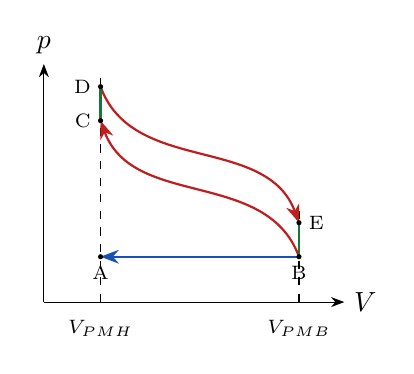
\begin{tikzpicture}[scale=0.72, >=Stealth]
\draw[->] (0,0) -- (5.3,0) node[right] {$V$};
\draw[->] (0,0) -- (0,4.2) node[above] {$p$};
\coordinate (A) at (1,0.8); \coordinate (B) at (4.5,0.8);
\coordinate (C) at (1,3.2); \coordinate (D) at (1,3.8);
\coordinate (E) at (4.5,1.4);
\draw[dashed] (1,0) -- (1,4.0); \node[below] at (1,-0.15) {\scriptsize $V_{PMH}$};
\draw[dashed] (4.5,0) -- (4.5,1.7); \node[below] at (4.5,-0.15) {\scriptsize $V_{PMB}$};
\draw[thick,crouge,->] (B) to[out=110,in=-70] (C);
\draw[thick,crouge,->] (D) to[out=-70,in=110] (E);
\draw[thick,cvert] (C) -- (D);
\draw[thick,cvert] (E) -- (B);
\draw[thick,cbleu,->] (B) -- (A);
\foreach \p/\lab/\pos in {A/A/below,B/B/below,C/C/left,D/D/left,E/E/right}
  {\fill (\p) circle (1.3pt) node[\pos] {\scriptsize\lab};}
\end{tikzpicture}
\end{center}

\begin{center}\small
\begin{tabularx}{0.85\linewidth}{@{}l l X@{}}
\toprule
B$\to$C & \textcolor{crouge}{adiabatique} & compression, rapide : $Q=0$ \\
C$\to$D & \textcolor{cvert}{isochore} & explosion (bougie), instantanée : $V$ ne bouge pas \\
D$\to$E & \textcolor{crouge}{adiabatique} & détente = temps moteur \\
E$\to$B & \textcolor{cvert}{isochore} & ouverture soupape, chute de $p$ \\
B$\to$A & \textcolor{cbleu}{isobare} & échappement (s'annule avec l'admission A$\to$B) \\
\bottomrule
\end{tabularx}
\end{center}

\etape{Les volumes (le seul endroit où $\varepsilon$ sert géométriquement)}
\pq{on connaît la cylindrée (le volume balayé) et le rapport $\varepsilon$ : deux équations, deux
inconnues $V_A$ et $V_B$.}

Cylindrée \textbf{par cylindre} : $\ \dfrac{1{,}2}{4}=0{,}3$ L. On écrit le système :
\[\begin{cases} V_B-V_A=0{,}3 \text{ L} \\[2pt] \dfrac{V_B}{V_A}=\varepsilon=10 \end{cases}
\ \Longrightarrow\ V_A\,(10-1)=0{,}3 \ \Longrightarrow\
\boxed{V_A=\frac{0{,}3}{9}=0{,}0333\text{ L}=3{,}333\cdot10^{-5}\text{ m}^3}\]
\[\boxed{V_B=10\,V_A=0{,}3333\text{ L}=3{,}333\cdot10^{-4}\text{ m}^3}\]
Et comme C et D sont au PMH : $V_C=V_D=V_A$. Comme E est au PMB : $V_E=V_B$.

\etape{Le point B (état connu) et la quantité de matière $n$}
\pq{B est le seul point dont on connaît directement $p$ et $T$ (c'est l'air ambiant aspiré). $n$ se
calcule là et servira pour TOUS les autres points, car la masse enfermée ne change plus.}

$T_B=16+273{,}15=289{,}15$ K, $\ p_B=1$ bar $=10^5$ Pa.
\[n=\frac{p_BV_B}{RT_B}=\frac{10^5\times3{,}333\cdot10^{-4}}{8{,}314\times289{,}15}
=\frac{33{,}33}{2403{,}6}=\boxed{0{,}013866\text{ mol}}\]

\etape{Le point C par la compression adiabatique}
\pq{B$\to$C est adiabatique réversible : on utilise $TV^{\gamma-1}=$ cste et $pV^\gamma=$ cste. Comme
$V_B/V_C=\varepsilon$, tout s'exprime avec $\varepsilon$.}

\[T_C=T_B\left(\frac{V_B}{V_C}\right)^{\gamma-1}=T_B\,\varepsilon^{\gamma-1}
=289{,}15\times10^{0,4}=289{,}15\times2{,}5119=\boxed{726{,}31\text{ K}}\]
\[p_C=p_B\,\varepsilon^{\gamma}=1\times10^{1,4}=\boxed{25{,}12\text{ bar}}\]

\etape{La combustion : de la formule chimique à $Q_{CD}$}
\pq{c'est la partie « chimie » de l'exercice. But : savoir quelle masse de carburant a été admise dans
le cylindre, pour en déduire la chaleur dégagée avec le PCI.}

\textbf{(a) Équilibrer la combustion} avec $C_xH_y+\left(x+\frac{y}{4}\right)O_2\to xCO_2+\frac{y}{2}H_2O$.
Ici $x=1$, $y=1{,}8$ :
\[CH_{1,8}+\underbrace{\left(1+\tfrac{1,8}{4}\right)}_{=1,45}O_2\ \longrightarrow\ CO_2+0{,}9\,H_2O\]

\textbf{(b) Passer de l'O$_2$ à l'air} (l'air ne contient que 21 \% d'O$_2$) :
\[n_{air,\text{stoe}}=\frac{1{,}45}{0{,}21}=6{,}905\ \text{mol d'air / mol de carburant}\]

\textbf{(c) Appliquer l'excès d'air} $\lambda=1{,}2$ :
\[n_{air,\text{r\'eel}}=1{,}2\times6{,}905=8{,}286\ \text{mol d'air / mol de carburant}\]

\textbf{(d) Répartir les $n$ moles du cylindre.} Le cylindre contient le mélange air + carburant, donc
pour 1 mole de carburant il y a $(8{,}286+1)=9{,}286$ moles de mélange :
\[n_{carb}=\frac{n}{9{,}286}=\frac{0{,}013866}{9{,}286}=1{,}4932\cdot10^{-3}\text{ mol}\]

\textbf{(e) Convertir en masse} ($M_{CH_{1,8}}=12\times1+1{,}8=13{,}8$ g/mol) :
\[m_{carb}=1{,}4932\cdot10^{-3}\times13{,}8=0{,}02061\text{ g}=2{,}061\cdot10^{-5}\text{ kg}\]

\textbf{(f) Chaleur de combustion} :
\[Q_{CD}=m_{carb}\cdot PCI=2{,}061\cdot10^{-5}\times42{,}5\cdot10^{6}=\boxed{875{,}8\text{ J}}\]

\begin{piege}
Attention à l'unité du PCI : $42500$ kJ/kg $=42{,}5\cdot10^6$ J/kg. Oublier ce facteur 1000 est
l'erreur la plus fréquente de tout l'exercice.
\end{piege}

\etape{Le point D par la combustion isochore}
\pq{C$\to$D est isochore, donc $W=0$ et toute la chaleur part dans l'énergie interne :
$Q=\Delta U=nC_v\Delta T$. On inverse cette relation pour trouver $T_D$.}

On calcule d'abord $nC_v=0{,}013866\times20{,}785=0{,}2882$ J/K, puis :
\[T_D=T_C+\frac{Q_{CD}}{nC_v}=726{,}31+\frac{875{,}8}{0{,}2882}=726{,}31+3038{,}8=\boxed{3765{,}1\text{ K}}\]
\[p_D=p_C\cdot\frac{T_D}{T_C}=25{,}12\times\frac{3765{,}1}{726{,}31}=\boxed{130{,}2\text{ bar}}
\quad(\text{isochore : } p/T \text{ constant})\]

\etape{Le point E par la détente adiabatique}
\pq{D$\to$E est adiabatique et ramène au PMB, donc $V_E=V_B$ et le rapport de volumes est encore
$\varepsilon$, mais en sens inverse.}
\[T_E=T_D\left(\frac{V_D}{V_E}\right)^{\gamma-1}=T_D\,\varepsilon^{1-\gamma}
=3765{,}1\times0{,}39811=\boxed{1498{,}9\text{ K}}\]
\[p_E=\frac{nRT_E}{V_B}=\frac{0{,}013866\times8{,}314\times1498{,}9}{3{,}333\cdot10^{-4}}
=\boxed{5{,}18\text{ bar}}\]

\etape{Les travaux et chaleurs de chaque transformation}
\pq{système fermé (gaz enfermé dans le cylindre) $\Rightarrow$ on utilise $\Delta U=W+Q$ et $C_v$
partout. Sur une adiabatique $Q=0$ donc $W=\Delta U$ ; sur une isochore $W=0$ donc $Q=\Delta U$.}

\begin{center}\small
\renewcommand{\arraystretch}{1.6}
\begin{tabularx}{\linewidth}{@{}l l X r@{}}
\toprule
\textbf{Transfo} & \textbf{Type} & \textbf{Calcul} & \textbf{Résultat} \\
\midrule
B$\to$C & adiab. & $W=nC_v(T_C-T_B)=0{,}2882\times(726{,}31-289{,}15)$ & $+126{,}0$ J \\
C$\to$D & isoch. & $W=0$ ; $Q=Q_{CD}$ (donné par la combustion) & $+875{,}8$ J \\
D$\to$E & adiab. & $W=nC_v(T_E-T_D)=0{,}2882\times(1498{,}9-3765{,}1)$ & $-653{,}1$ J \\
E$\to$B & isoch. & $W=0$ ; $Q=nC_v(T_B-T_E)=0{,}2882\times(289{,}15-1498{,}9)$ & $-348{,}7$ J \\
\midrule
\textbf{Cycle} & & $W_{cycle}=126{,}0-653{,}1$ & $\mathbf{-527{,}1}$ \textbf{J} \\
\bottomrule
\end{tabularx}
\end{center}

\begin{verif}
\textbf{Vérification obligatoire} (elle vous sauve d'une erreur de signe) : sur un cycle,
$\Delta U=0$ donc la somme de tout doit être nulle :
\[Q_{CD}+Q_{EB}+W_{cycle}=875{,}8-348{,}7-527{,}1=0\quad\checkmark\]
Et $W_{cycle}<0$ : le cycle \textbf{fournit} du travail, c'est bien un moteur. \checkmark
\end{verif}

\etape{Le rendement théorique}
\pq{deux chemins mènent au même résultat : la formule toute faite, ou le rapport des énergies déjà
calculées. Faites les deux, c'est votre contrôle.}

\textbf{Par la formule :}
\[\eta_{th}=1-\varepsilon^{1-\gamma}=1-10^{-0,4}=1-0{,}39811=\boxed{0{,}6019=60{,}19\ \%}\]
\textbf{Par les énergies :} $\ \eta_{th}=\dfrac{|W_{cycle}|}{Q_{CD}}=\dfrac{527{,}1}{875{,}8}=0{,}6019$
\checkmark

\etape{Les rendements en cascade}
\pq{le cycle réel ne suit pas les courbes théoriques ($\eta_f$) et il y a des frottements
($\eta_{m\acute{e}ca}$). On applique les pertes l'une après l'autre.}
\[|W_{th}|=527{,}1\text{ J}
\ \xrightarrow{\ \times\,0,75\ }\ |W_{ind}|=395{,}4\text{ J}
\ \xrightarrow{\ \times\,0,8\ }\ |W_{dispo}|=\boxed{316{,}3\text{ J}}\]
Rendement effectif global : $\eta_{eff}=0{,}6019\times0{,}75\times0{,}8=0{,}3611=36{,}1\ \%$.

\etape{La vitesse de rotation}
\pq{$W_{dispo}$ est le travail d'\textbf{un} cylindre pour \textbf{un} cycle. Pour une puissance, il faut
le nombre de cycles par seconde ($N/60$ tours par seconde, et 1 cycle = 2 tours en 4 temps) fois le
nombre de cylindres.}
\[P_{eff}=\frac{N}{2\times60}\,|W_{dispo}|\,z
\ \Longrightarrow\
N=\frac{P_{eff}\times120}{|W_{dispo}|\times z}=\frac{20\,000\times120}{316{,}3\times4}
=\frac{2\,400\,000}{1265{,}1}=\boxed{1897\text{ tr/min}}\]

\begin{piege}
\textbf{En 2 temps}, 1 cycle $=$ 1 tour : la formule devient $P=\frac{N}{60}\,W\,z$ (pas de division
par 2). Tout le reste du calcul est \textbf{identique} à l'essence.
\end{piege}

\newpage
%=====================================================
\section{Moteur diesel : ce qui change}

\begin{enonce}
\textbf{Énoncé.} Diesel 4 temps, 4 cylindres, cylindrée 2 L, $\varepsilon=18$, rapport de combustion
$\rho=2$. Air admis à $27\,^\circ$C et 1 bar, $\gamma=1{,}4$. $N=2200$ tr/min.
\emph{Trouver les points, le rendement théorique et la puissance.}
\end{enonce}

\begin{reflexe}
\textbf{Une seule différence de fond avec l'essence :} la combustion C$\to$D est \textbf{isobare} (le
carburant est injecté progressivement) au lieu d'être isochore. Conséquences en chaîne :
\begin{itemize}[leftmargin=1.3em,nosep]
\item $V_D\neq V_C$ : il faut le nouveau paramètre $\rho=V_D/V_C$ ;
\item la chaleur de combustion utilise $C_p$ et non $C_v$ ;
\item le rendement a une formule plus lourde, avec $\rho$ ;
\item la détente D$\to$E ne part plus du PMH, le rapport de volumes devient $\rho/\varepsilon$.
\end{itemize}
Tout le reste (volumes, $n$, compression, échappement, puissance) est \textbf{identique}.
\end{reflexe}

\etape{Volumes}
$V_A=\dfrac{2/4}{18-1}=\dfrac{0{,}5}{17}=0{,}02941$ L $=2{,}941\cdot10^{-5}$ m$^3$ ;
$\ V_B=18\,V_A=0{,}5294$ L.
\textbf{Nouveau :} $V_D=\rho\,V_C=2\times0{,}02941=0{,}05882$ L.

\etape{Point B et $n$}
$T_B=300{,}15$ K, $p_B=10^5$ Pa :
\[n=\frac{10^5\times5{,}294\cdot10^{-4}}{8{,}314\times300{,}15}=\boxed{0{,}021215\text{ mol}}\]

\etape{Point C (compression adiabatique -- identique à l'essence)}
\[T_C=300{,}15\times18^{0,4}=300{,}15\times3{,}1777=\boxed{953{,}8\text{ K}}
\qquad p_C=18^{1,4}=\boxed{57{,}2\text{ bar}}\]

\etape{Point D par la combustion ISOBARE}
\pq{à pression constante, la loi des gaz parfaits donne directement $V/T$ constant : le rapport des
volumes $\rho$ EST le rapport des températures. C'est beaucoup plus simple que pour l'essence.}
\[\frac{T_D}{T_C}=\frac{V_D}{V_C}=\rho \ \Longrightarrow\
T_D=2\times953{,}8=\boxed{1907{,}6\text{ K}}\qquad p_D=p_C=\boxed{57{,}2\text{ bar}}\]
La chaleur apportée se calcule alors avec $C_p$ (transformation isobare) :
\[Q_{CD}=nC_p(T_D-T_C)=0{,}021215\times29{,}099\times(1907{,}6-953{,}8)=0{,}6173\times953{,}8
=\boxed{588{,}8\text{ J}}\]

\etape{Point E par la détente adiabatique}
\pq{la détente part de $V_D=\rho V_A$ et finit à $V_B=\varepsilon V_A$ : le rapport de volumes vaut donc
$\rho/\varepsilon$, et non $1/\varepsilon$ comme pour l'essence.}
\[\frac{V_D}{V_E}=\frac{\rho}{\varepsilon}=\frac{2}{18}=\frac{1}{9}\]
\[T_E=T_D\left(\frac19\right)^{0,4}=1907{,}6\times0{,}41524=\boxed{792{,}1\text{ K}}
\qquad p_E=p_D\left(\frac19\right)^{1,4}=57{,}2\times0{,}046138=\boxed{2{,}64\text{ bar}}\]

\etape{Rendement théorique}
\pq{la formule est longue : calculez les morceaux séparément et notez-les, sinon vous vous perdez.}
\[\eta_{th}=1+\frac{\varepsilon^{1-\gamma}-\varepsilon^{1-\gamma}\rho^{\gamma}}{\gamma(\rho-1)}\]
Morceau par morceau : $\varepsilon^{1-\gamma}=18^{-0,4}=0{,}3147$ ; $\ \rho^{\gamma}=2^{1,4}=2{,}639$ ;
$\ \gamma(\rho-1)=1{,}4\times1=1{,}4$.
\[\eta_{th}=1+\frac{0{,}3147-0{,}3147\times2{,}639}{1{,}4}
=1+\frac{0{,}3147-0{,}8305}{1{,}4}=1-\frac{0{,}5158}{1{,}4}=1-0{,}3684=\boxed{0{,}6316=63{,}16\ \%}\]

\etape{Travail et puissance}
\[|W_{th}|=\eta_{th}\cdot Q_{CD}=0{,}6316\times588{,}8=\boxed{371{,}9\text{ J}}\]
\[P_{th}=\frac{N}{120}\,|W_{th}|\,z=\frac{2200}{120}\times371{,}9\times4
=18{,}33\times371{,}9\times4=\boxed{27{,}3\text{ kW}}\]

\begin{verif}
\textbf{Contrôle par les travaux détaillés} (à faire si vous avez le temps) :
$W_{BC}=nC_v(T_C-T_B)=+288{,}2$ J ; $W_{CD}=-p_C(V_D-V_C)=-168{,}2$ J (isobare, le gaz pousse le
piston) ; $W_{DE}=nC_v(T_E-T_D)=-491{,}9$ J.
\[W_{cycle}=288{,}2-168{,}2-491{,}9=-371{,}9\text{ J}\quad\checkmark\ \text{(même valeur, signe négatif
= moteur)}\]
\end{verif}

\begin{piege}
$\varepsilon$ pour un diesel vaut 16 à 20 (contre 8 à 10 pour l'essence) : si vous trouvez
$\varepsilon=10$ sur un diesel, vous vous êtes trompé quelque part. De même $T_C$ doit être très élevée
($\sim950$ K) : c'est ce qui permet l'auto-inflammation sans bougie.
\end{piege}

\newpage
%=====================================================
\section{Machine frigorifique / pompe à chaleur}

\begin{enonce}
\textbf{Énoncé.} PAC au R134a. Évaporation à $-5\,^\circ$C, condensation à $45\,^\circ$C, surchauffe et
sous-refroidissement de $5\,^\circ$C. Rendement isentropique du compresseur $\eta_{isos}=0{,}75$.
Lecture sur le diagramme : $h_{1'}=402{,}5$ ; $h_{2s}=435$ ; $h_{3'}=257$ kJ/kg. La maison perd 12 kW.
L'eau des radiateurs passe de 35 à $40\,^\circ$C ($c=4185$ J/kg$\cdot$K).
\emph{Trouver le COP, le débit de fluide, la puissance du compresseur, le débit d'eau.}
\end{enonce}

\begin{reflexe}
\textbf{Changement de logique par rapport aux moteurs :} ici le fluide \textbf{traverse} des machines
(système \textbf{ouvert}) $\Rightarrow$ on travaille avec des \textbf{enthalpies} $h$ lues sur le
diagramme, pas avec $C_v$ et des températures. Aucun calcul de $pV=nRT$ dans cet exercice.
\end{reflexe}

\etape{Placer les 4 points sur le diagramme $(\log p,h)$}
\pq{les enthalpies ne se calculent pas, elles se LISENT. Le travail de l'exercice consiste surtout à
placer correctement les points.}

\begin{center}
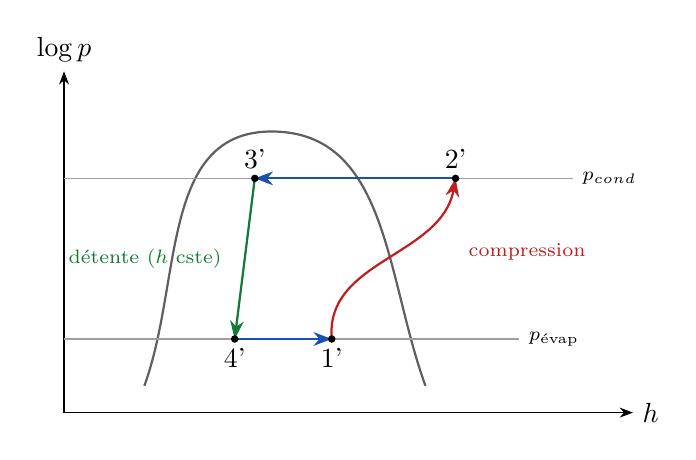
\begin{tikzpicture}[scale=0.85, >=Stealth]
\draw[->] (0,0) -- (8.5,0) node[right] {$h$};
\draw[->] (0,0) -- (0,5.1) node[above] {$\log p$};
\draw[thick,cgris] (1.2,0.4) to[out=70,in=180] (3.1,4.2) to[out=0,in=110] (5.4,0.4);
\draw[cgris!60] (0,3.5) -- (7.6,3.5) node[right,black]{\scriptsize $p_{cond}$};
\draw[cgris!60] (0,1.1) -- (6.8,1.1) node[right,black]{\scriptsize $p_{\text{\'evap}}$};
\coordinate (p4) at (2.55,1.1); \coordinate (p1) at (4.0,1.1);
\coordinate (p2) at (5.85,3.5); \coordinate (p3) at (2.85,3.5);
\draw[thick,crouge,->] (p1) to[out=95,in=-100] (p2);
\draw[thick,cbleu,->] (p2) -- (p3);
\draw[thick,cvert,->] (p3) -- (p4);
\draw[thick,cbleu,->] (p4) -- (p1);
\foreach \p/\lab/\pos in {p1/1'/below,p2/2'/above,p3/3'/above,p4/4'/below}
  {\fill (\p) circle (1.6pt) node[\pos] {\lab};}
\node[crouge,right] at (5.9,2.4) {\scriptsize compression};
\node[cvert,left] at (2.5,2.3) {\scriptsize détente ($h$ cste)};
\end{tikzpicture}
\end{center}

\begin{center}\small
\begin{tabularx}{0.92\linewidth}{@{}l X@{}}
\toprule
\textbf{1'} & sur l'isobare BP, à $T_{\text{\'evap}}+5=-5+5=0\,^\circ$C (surchauffe) $\rightarrow$ zone
vapeur, à droite de la cloche \\
\textbf{2'} & sur l'isobare HP, en suivant l'\textbf{isentropique} partant de 1' \\
\textbf{3'} & sur l'isobare HP, à $T_{cond}-5=45-5=40\,^\circ$C (sous-refroidissement) $\rightarrow$
zone liquide, à gauche \\
\textbf{4'} & \textbf{à la verticale de 3'} (détente isenthalpique : $h_{4'}=h_{3'}$) \\
\bottomrule
\end{tabularx}
\end{center}

\etape{Corriger le point 2 (compresseur réel)}
\pq{le diagramme donne le point idéal $2s$ (isentropique). Le compresseur réel consomme plus, donc le
point réel est plus à droite. $\eta_{isos}$ fait le lien.}
\[\eta_{isos}=\frac{h_{2s}-h_1}{h_{2}-h_1}
\ \Longrightarrow\ h_2=h_1+\frac{h_{2s}-h_1}{\eta_{isos}}
=402{,}5+\frac{435-402{,}5}{0{,}75}=402{,}5+43{,}33=\boxed{445{,}83\text{ kJ/kg}}\]
Et par la détente isenthalpique : $\ \boxed{h_4=h_3=257\text{ kJ/kg}}$.

\etape{Les trois énergies par kilogramme}
\pq{chaque machine ouverte adiabatique donne $w_{ut}=\Delta h$, et chaque échangeur isobare donne
$q=\Delta h$. Donc tout se lit comme des différences d'enthalpie, dans le sens du parcours.}

\begin{center}\small
\renewcommand{\arraystretch}{1.6}
\begin{tabularx}{\linewidth}{@{}l l X r@{}}
\toprule
\textbf{Étape} & \textbf{Organe} & \textbf{Calcul} & \textbf{Résultat} \\
\midrule
1$\to$2 & compresseur & $w=h_2-h_1=445{,}83-402{,}5$ & $+43{,}33$ kJ/kg \\
2$\to$3 & condenseur & $q_1=h_3-h_2=257-445{,}83$ & $-188{,}83$ kJ/kg \\
3$\to$4 & détendeur & $h$ constante & $0$ \\
4$\to$1 & évaporateur & $q_2=h_1-h_4=402{,}5-257$ & $+145{,}50$ kJ/kg \\
\bottomrule
\end{tabularx}
\end{center}

\begin{verif}
\textbf{Vérification} : sur un cycle, $q_1+q_2+w=0$ :
\[-188{,}83+145{,}50+43{,}33=0\quad\checkmark\]
Signes cohérents : $w>0$ (on fournit du travail), $q_1<0$ (on cède au chaud), $q_2>0$ (on prend au
froid). \checkmark
\end{verif}

\etape{COP ou PSN ? (la question à se poser)}
\pq{la formule dépend de ce qu'on cherche à obtenir. C'est ici qu'on perd des points si on récite sans
réfléchir.}

\begin{center}\small
\begin{tabularx}{0.95\linewidth}{@{}l X l@{}}
\toprule
\textbf{Machine} & \textbf{Ce qui est utile} & \textbf{Formule} \\
\midrule
Frigo & la chaleur \emph{prise} au froid & $PSN=\dfrac{q_2}{w}$ \\
PAC (ici) & la chaleur \emph{cédée} au chaud & $COP=\dfrac{-q_1}{w}$ \\
\bottomrule
\end{tabularx}
\end{center}
Ici c'est une PAC qui chauffe une maison :
\[COP=\frac{-q_1}{w}=\frac{188{,}83}{43{,}33}=\boxed{4{,}36}\]

\begin{verif}
\textbf{Contrôle de vraisemblance par Carnot} (avec les températures des \textbf{sources}, en K) :
\[COP_{max}=\frac{T_1}{T_1-T_2}=\frac{318{,}15}{318{,}15-268{,}15}=\frac{318{,}15}{50}=6{,}36\]
Notre COP réel ($4{,}36$) vaut 69 \% du maximum : c'est réaliste. S'il était \emph{supérieur} à
$COP_{max}$, il y aurait une erreur.
\end{verif}

\etape{Passer aux puissances et aux débits}
\pq{jusqu'ici tout était « par kg ». Le débit est le pont entre les kJ/kg et les kW.}

La maison a besoin de 12 kW, fournis par le \textbf{condenseur} (c'est lui qui chauffe) :
\[\dot m=\frac{P_{utile}}{|q_1|}=\frac{12}{188{,}83}=\boxed{0{,}0636\text{ kg/s}}\]
\[P_{comp}=\dot m\cdot w=0{,}0636\times43{,}33=\boxed{2{,}75\text{ kW}}\]

\begin{verif}
$P_{\text{\'evap}}=\dot m\cdot q_2=0{,}0636\times145{,}5=9{,}25$ kW, et
$2{,}75+9{,}25=12{,}0$ kW \checkmark : la chaleur donnée à la maison = celle prise dehors (gratuite) +
le travail électrique payé. C'est tout l'intérêt d'une PAC.
\end{verif}

\etape{Le circuit d'eau (partie « échange thermique »)}
\pq{c'est un fluide qui ne change pas de phase : on quitte les enthalpies du diagramme et on revient à
la formule de calorimétrie. Le lien entre les deux circuits est la \textbf{puissance}, identique des
deux côtés de l'échangeur.}
\[P=\dot m_{eau}\,c\,\Delta T
\ \Longrightarrow\
\dot m_{eau}=\frac{P}{c\,\Delta T}=\frac{12\,000}{4185\times5}=\frac{12\,000}{20\,925}
=\boxed{0{,}573\text{ kg/s}}\ (\approx2{,}06\text{ m}^3/\text{h})\]

\newpage
%=====================================================
\section{Turbine à gaz (cycle de Joule)}

\begin{enonce}
\textbf{Énoncé.} Air ($c_p=1004$ J/kg$\cdot$K, $\gamma=1{,}4$), débit $35$ kg/s.
1-2 : compression adiabatique de 1 à $4{,}1$ atm, $T_1=15\,^\circ$C. 2-3 : échauffement isobare jusqu'à
$750\,^\circ$C. 3-4 : détente adiabatique dans une turbine dont \textbf{tout le travail sert à entraîner
le compresseur}. 4-5 : échauffement isobare jusqu'à $700\,^\circ$C. 5-6 : détente adiabatique jusqu'à
1 atm. 6-1 : refroidissement isobare.
\emph{Trouver $T_2$, $T_4$, $T_6$, $p_4$, le rendement, la puissance utile.}
\end{enonce}

\begin{reflexe}
\textbf{Machines ouvertes} $\Rightarrow$ $c_p$ partout et raisonnement \textbf{par kg} (pas de moles,
pas de volumes). Le débit n'intervient qu'à la toute fin pour convertir en watts.
Formules de base : adiabatique $\rightarrow w=c_p\Delta T$ et $Q=0$ ; isobare $\rightarrow q=c_p\Delta T$
et $w_{ut}=0$.
\end{reflexe}

\etape{Point 2 : compression adiabatique avec un rapport de pression}
\pq{on ne connaît que les pressions, donc on prend la forme de l'adiabatique reliant $T$ et $p$.}
\[T_2=T_1\left(\frac{p_2}{p_1}\right)^{\frac{\gamma-1}{\gamma}}
=288{,}15\times(4{,}1)^{0,2857}=288{,}15\times1{,}4965=\boxed{431{,}2\text{ K}}\]
Travail du compresseur : $\ w_{12}=c_p(T_2-T_1)=1004\times143{,}07=+143{,}6$ kJ/kg.

\etape{Point 3 : échauffement isobare (donné)}
$T_3=750+273{,}15=1023{,}15$ K, $p_3=p_2=4{,}1$ atm.
\[q_{23}=c_p(T_3-T_2)=1004\times(1023{,}15-431{,}22)=1004\times591{,}93=+594{,}3\text{ kJ/kg}\]

\etape{Point 4 : la turbine qui entraîne le compresseur}
\pq{c'est LA subtilité de l'exercice. « Tout le travail sert au compresseur » signifie que le travail de
la turbine est l'opposé de celui du compresseur. Comme le débit est le même partout, on peut écrire
l'égalité directement sur les $\Delta T$.}
\[|w_{34}|=|w_{12}| \ \Longrightarrow\ c_p(T_3-T_4)=c_p(T_2-T_1)
\ \Longrightarrow\ T_3-T_4=T_2-T_1\]
\[T_4=T_3-(T_2-T_1)=1023{,}15-(431{,}22-288{,}15)=1023{,}15-143{,}07=\boxed{880{,}1\text{ K}}\]
La pression $p_4$ vient ensuite de l'adiabatique 3-4 :
\[p_4=p_3\left(\frac{T_4}{T_3}\right)^{\frac{\gamma}{\gamma-1}}
=4{,}1\times(0{,}8602)^{3,5}=4{,}1\times0{,}5902=\boxed{2{,}42\text{ atm}}\]

\etape{Points 5 et 6}
$T_5=700+273{,}15=973{,}15$ K (isobare, $p_5=p_4=2{,}42$ atm) :
\[q_{45}=c_p(T_5-T_4)=1004\times(973{,}15-880{,}08)=+93{,}4\text{ kJ/kg}\]
Détente finale jusqu'à $p_6=p_1=1$ atm :
\[T_6=T_5\left(\frac{p_6}{p_5}\right)^{0,2857}=973{,}15\times\left(\frac{1}{2{,}42}\right)^{0,2857}
=973{,}15\times0{,}7769=\boxed{756{,}0\text{ K}}\]
\[w_{56}=c_p(T_6-T_5)=1004\times(756{,}0-973{,}15)=\boxed{-218{,}0\text{ kJ/kg}}\]

\etape{Rendement}
\pq{le travail « net » n'est PAS la somme de toutes les turbines : celui de la première est entièrement
consommé par le compresseur, il ne sort pas de la machine. Seule la seconde turbine produit de l'utile.}
\[W_{net}=\underbrace{+143{,}6}_{\text{compresseur}}\underbrace{-143{,}6}_{\text{turbine 1}}
\underbrace{-218{,}0}_{\text{turbine 2}}=-218{,}0\text{ kJ/kg}\]
\[Q_{fourni}=q_{23}+q_{45}=594{,}3+93{,}4=687{,}7\text{ kJ/kg}\]
\[\eta=\frac{|W_{net}|}{Q_{fourni}}=\frac{218{,}0}{687{,}7}=\boxed{0{,}317=31{,}7\ \%}\]

\etape{Puissance}
\[P=\dot m\cdot W_{net}=35\times(-218{,}0)=\boxed{-7630\text{ kW}=-7{,}63\text{ MW}}\]
\emph{Le signe négatif est normal : la machine \textbf{fournit} de l'énergie à l'extérieur.}

\begin{verif}
\textbf{Vraisemblance :} $\eta_{Carnot}$ entre la source froide ($288{,}15$ K) et la plus haute
température ($1023{,}15$ K) vaut $1-\frac{288{,}15}{1023{,}15}=71{,}8\ \%$. Nos $31{,}7\ \%$ sont bien
en dessous : cohérent. Un rendement au-dessus de Carnot signalerait une erreur.
\end{verif}

\newpage
%=====================================================
\section{Les 6 vérifications qui rattrapent une erreur}

\begin{reflexe}
Avant de rendre, passez cette liste sur chaque exercice. Chacune prend 10 secondes et peut sauver
plusieurs points.
\end{reflexe}

\begin{center}
\renewcommand{\arraystretch}{1.7}
\begin{tabularx}{\linewidth}{@{}c X@{}}
\toprule
\textbf{1} & \textbf{Toutes les températures sont-elles en Kelvin ?} Une seule oubliée en $^\circ$C
fausse tout le reste. \\
\textbf{2} & \textbf{La somme sur le cycle est-elle nulle ?} $\sum W+\sum Q=0$ (car $\Delta U_{cycle}=0$).
C'est la vérification la plus puissante : elle teste tous vos calculs d'un coup. \\
\textbf{3} & \textbf{Le signe du travail correspond-il au type de machine ?} Moteur $\rightarrow
W_{cycle}<0$ ; frigo/PAC $\rightarrow W>0$. \\
\textbf{4} & \textbf{Le rendement est-il en dessous de Carnot ?} $\eta<\eta_{Carnot}=1-T_2/T_1$, et
$COP<COP_{max}=\frac{T_1}{T_1-T_2}$. Sinon, erreur garantie. \\
\textbf{5} & \textbf{Les deux chemins donnent-ils le même rendement ?} La formule
($1-\varepsilon^{1-\gamma}$) doit redonner $|W_{cycle}|/Q_{fourni}$. \\
\textbf{6} & \textbf{Les ordres de grandeur sont-ils crédibles ?} $T$ après combustion : 2000--3800 K ;
$p_{max}$ : quelques dizaines à $\sim$130 bar ; $\eta$ moteur : 30--65 \% ; $COP$ d'une PAC : 3--5 ;
$N$ : 1000--6000 tr/min. \\
\bottomrule
\end{tabularx}
\end{center}

\section*{Récapitulatif : quelle formule pour quel cas}
\addcontentsline{toc}{section}{Récapitulatif : quelle formule pour quel cas}

\begin{center}
\renewcommand{\arraystretch}{1.6}
\begin{tabularx}{\linewidth}{@{}l l X@{}}
\toprule
\textbf{Situation} & \textbf{Système} & \textbf{Ce que j'utilise} \\
\midrule
Gaz enfermé dans un cylindre & fermé & $\Delta U=W+Q$, \ $\Delta U=nC_v\Delta T$, \ $W=-\int p\,dV$ \\
Fluide qui traverse une machine & ouvert & $\Delta H=W_{ut}+Q$, \ $\Delta H=nC_p\Delta T$ (ou $\Delta h$
lu au diagramme) \\
Compression / détente rapide & --- & adiabatique : $Q=0$, \ $TV^{\gamma-1}=T^{\gamma}p^{1-\gamma}=pV^{\gamma}=$ cste \\
Explosion essence, échappement & --- & isochore : $W=0$, \ $Q=nC_v\Delta T$, \ $p/T$ cste \\
Combustion diesel, échangeur & --- & isobare : $Q=nC_p\Delta T$, \ $V/T$ cste \\
Soupape de détente (frigo) & ouvert & isenthalpique : $h_4=h_3$ \\
Eau, air d'un local (sans changement d'état) & --- & $Q=mc\Delta T$ \ ou \ $P=\dot m\,c\,\Delta T$ \\
\bottomrule
\end{tabularx}
\end{center}

\end{document}
